\documentclass[a4paper,UTF8]{article}
\usepackage{ctex}
\usepackage[margin=1.25in]{geometry}
\usepackage{color}
\usepackage{graphicx}
\usepackage{amssymb}
\usepackage{amsmath}
\usepackage{amsthm}
\usepackage{soul, color, xcolor}
\usepackage{bm}
\usepackage{tcolorbox}
\usepackage{hyperref}
\numberwithin{equation}{section}
%\usepackage[thmmarks, amsmath, thref]{ntheorem}
\theoremstyle{definition}
\newtheorem*{solution}{Solution}
\newtheorem*{prove}{Proof}
\usepackage{multirow}
\usepackage{diagbox}
\usepackage{float}

\setlength{\parindent}{0pt}
\newcommand{\bds}{\boldsymbol}
\def \X {\mathbf{X}}
\def \A {\mathbf{A}}
\def \C {\mathbf{C}}
\def \w {\hat{\boldsymbol{w}}}
\def \y {\mathbf{y}}
\def \x {\mathbf{x}}
\def \z {\mathbf{z}}
\def \hy {\widehat{y}}
\def \by {\Bar{y}}
\def \H {\mathbf{H}}
\def \I {\mathbf{I}}
\newcommand\given[1][]{\:#1\vert\:}


\begin{document}
\title{机器学习导论\ 习题二}
\author{211300063, 张运吉, \href{mailto:邮箱}{211300063@smail.nju.edu.cn}}
\maketitle
\section*{作业提交注意事项}
\begin{tcolorbox}
	\begin{enumerate}
		\item[1.] 请在LaTeX模板中第一页填写个人的学号、姓名、邮箱;
		\item[2.] 本次作业需提交作答后的该 pdf 文件、编程题~.ipynb 文件; {\color{red}\textbf{请将二者打包为~.zip 文件上传}}. 注意命名规则, 三个文件均命名为 “$\text{学号}\_\text{姓名}$” + “.后缀” (例如 $\text{211300001}\_\text{张三}$” + “.pdf”、“.ipynb”、“.zip”);
		\item[3.] 若多次提交作业, 则在命名~.zip 文件时加上版本号, 例如 211300001\_张三\_v1.zip” (批改时以版本号最高的文件为准);
		\item[4.] 本次作业提交截止时间为 {\color{red}\textbf{ 4 月 19 日23:59:59}}. 未按照要求提交作业, 提交作业格式不正确, {\color{red}\textbf{作业命名不规范}}, 将会被扣除部分作业分数; 除特殊原因 (如因病缓交, 需出示医院假条) 逾期未交作业, 本次作业记 0 分; {\color{red}\textbf{如发现抄袭, 抄袭和被抄袭双方成绩全部取消}};
		\item[5.] 本次作业提交地址为 \href{https://box.nju.edu.cn/u/d/72f6f8cfff054611b6d3/}{here}, 请大家预留时间提前上交, 以防在临近截止日期时, 因网络等原因无法按时提交作业.
	\end{enumerate}
\end{tcolorbox}
\newpage


\section{[20pts] Linear Discriminant Analysis}
线性判别分析 (Linear Discriminant Analysis, 简称 LDA) 是一种经典的线性学习方法. 请仔细阅读《机器学习》第三章 3.4 节, 并回答如下问题.

\begin{enumerate}
	\item[(1)] \textbf{[10pts]} (二分类) 假设有两类数据, 其中正类服从高斯分布$P=\mathcal{N}\left(\bds{\mu}_1, \bds{\Sigma}_1\right)$, 负类服从高斯分布 $Q=\mathcal{N}\left(\bds{\mu}_2, \bds{\Sigma}_2\right)$. 对于任一样本 $\bds{x}$, 若分类器 $h$ 满足:
     $$
     h(\bds{x})= \begin{cases}0 & P(\bds{x})\leq Q(\bds{x}), \\ 1 & P(\bds{x})>Q(\bds{x}), \end{cases}
     $$
     则认为 $h$ 实现了最优分类. 假设 $\bds{\mu}_1,\bds{\mu}_2, \bds{\Sigma}_1, \bds{\Sigma}_2$ 均已知, 请证明当 $\bds{\Sigma}_1=\bds{\Sigma}_2=\bds{\Sigma}$ 时, 通过 LDA 得到的分类器可实现最优分类.
     (提示: 找到满足最优分类性质的分类平面)
	\item[(2)] \textbf{[10pts]} (多分类) 将 LDA 推广至多分类任务时, 可采用教材中式 (3.44) 作为优化目标. 通过求解式 (3.44), 可得到投影矩阵 $\mathbf{W}\in \mathbb{R}^{d\times d'}$, 其中 $d$ 为数据原有的属性数. 假设当前任务共有 $N$ 个类别, 请证明 $d'\leq N-1$. (提示: 对于任意 $n$ 阶方阵, 其非零特征值个数小于等于其秩大小)
\end{enumerate}


\begin{solution}
	此处用于写解答 (中英文均可)
	\begin{enumerate}
		\item[(1)]
		当$P(x) = Q(x)$时,
		$$\frac{1}{(2\pi)^{\frac{n}{2}}\bds{\Sigma}^{\frac{1}{2}}} exp\left({-\frac{1}{2}(\bds{x} - \bds{\mu}_1)^T\bds{\Sigma}^{-1}(\bds{x}-\bds{\mu}_1)} \right)= \frac{1}{(2\pi)^{\frac{n}{2}}\bds{\Sigma}^{\frac{1}{2}}} exp\left({-\frac{1}{2}(\bds{x} - \bds{\mu}_2)^T\bds{\Sigma}^{-1}(\bds{x}-\bds{\mu}_2)} \right)$$
		化简得:
		$$\bds{x}^T\bds{\Sigma}^{-1}(\bds{\mu}_2-\bds{\mu}_1) - \frac{1}{2}(\bds{\mu}_2+\bds{\mu}_1)^T\bds{\Sigma}^{-1}(\bds{\mu}_2-\bds{\mu}_1) = 0$$
		上式即为满足最优分类性质的分类平面。\\
		通过 LDA 得到的分类器:
		\begin{equation}
			\begin{split}
				\bds{w} &= \mathbf{S}_{w}^{-1}(\bds{\mu}_1-\bds{\mu}_2) \\
				&= (\bds{\Sigma}_1+\bds{\Sigma}_2)^{-1}(\bds{\mu}_1-\bds{\mu}_2) \\
				&= \frac{1}{2}\bds{\Sigma}^{-1}(\bds{\mu}_1-\bds{\mu}_2)
			\end{split}
			\notag
		\end{equation}
		两类样本投影中心 
		$$\bds{\mu}'_1 = \frac{1}{2}\bds{\mu}_1^T\bds{\Sigma}^{-1}(\bds{\mu}_1-\bds{\mu}_2)$$
		$$\quad \bds{\mu}'_2 = \frac{1}{2}\bds{\mu}_2^T\bds{\Sigma}^{-1}(\bds{\mu}_1-\bds{\mu}_2)$$
		分类点:
		\begin{equation}
			\begin{split}
				\bds{\mu}' &= \frac{1}{2}(\bds{\mu}'_1+\bds{\mu}'_2) \\
				&= \frac{1}{4}(\bds{\mu}_1+\bds{\mu}_2)^T\bds{\Sigma}^{-1}(\bds{\mu}_1-\bds{\mu}_2)
			\end{split}
			\notag
		\end{equation}
		所以由LDA得到的分类平面:
		$$\bds{x}^T\bds{w} - \bds{\mu}' = 0$$
		即:
		$$\bds{x}^T\bds{\Sigma}^{-1}(\bds{\mu}_2-\bds{\mu}_1) - \frac{1}{2}(\bds{\mu}_2+\bds{\mu}_1)^T\bds{\Sigma}^{-1}(\bds{\mu}_2-\bds{\mu}_1) = 0$$
		所以在 $\bds{\Sigma_1} = \bds{\Sigma_2} = \bds{\Sigma}$时,通过LDA得到的分类器可实现最优分类.
		\item[(2)] 
		由课本上定义:$\textbf{S}_b = \sum_{i=1}^{N}m_i(\bds{\mu}_i-\bds{\mu})(\bds{\mu}_i-\bds{\mu})^T$ 以及 $\text{rank }(m_i(\bds{\mu}_i-\bds{\mu})(\bds{\mu}_i-\bds{\mu})^T) \leq \min\{\bds{\mu}_i-\bds{\mu},(\bds{\mu}_i-\bds{\mu})^T\} = 1$ \\
		所以: $\text{rank }(\textbf{S}_b) \leq N$ \\
		因为一共有$N$个类别,所以第$N$个类别的均值$\mu_N$可以由前$N-1$个类别的均值线性表示,因此$A_N = m_N(\bds{\mu}_N-\bds{\mu})(\bds{\mu}_N-\bds{\mu})^T$可以由$A_i = m_i(\bds{\mu}_i-\bds{\mu})(\bds{\mu}_i-\bds{\mu})^T, i=0,1, ..., N-1$线性表示。\\
		所以: $\text{rank }(\textbf{S}_b) \leq N-1$ \\
		$\text{rank }(\textbf{S}_w^{-1}\textbf{S}_b) \leq \text{rank }(\textbf{S}_b) \leq N-1$ \\
		因为:对于任意 n 阶方阵, 其非零特征值个数小于等于其秩大小 \\
		所以:矩阵$\textbf{S}_w^{-1}\textbf{S}_b$的非零特征值个数$\leq N-1$ \\
		所以:$d^{'} \leq N-1$
	\end{enumerate}
\end{solution}

\newpage

\section{[20pts] Multi-Class Learning}
现实场景中我们经常会遇到多分类任务,处理思路主要分为两种:一是利用一些基本策略
(OvO,OvR,MvM),将多分类任务拆分为若干个二分类任务;二是直接求解,将常见的二分类学习器推广为多分类学习器. 请仔细阅读《机器学习》第三章3.5节,并回答如下问题.
\begin{enumerate}
	\item[(1)] \textbf{[5pts]}  考虑如下多分类学习问题:样本数量为$n$, 类别数量为$K$, 每个类别的样本数量一致. 假设一个二分类算法对于大小为$m$的数据训练的时间复杂度为$\mathcal{O}(m^\alpha)$, 试分别计算该算法在OvO、OvR策略下训练的总体时间复杂度.
	\item[(2)] \textbf{[5pts]}  当我们使用MvM处理多分类问题时,正、反类的构造需要有特殊的设计,一种最常用的技术是“纠错输出码"(ECOC). 考虑ECOC中的编码矩阵为“三元码”的形式,即在正、反类之外加入了“停用类”. 请通过构造具体的编码矩阵, 说明OvO、OvR均为此ECOC的特例.
	\item[(3)] \textbf{[10pts]}  对数几率回归(logistic regression)是一种常用的二分类模型, 简称对率回归. 现如今问题由二分类推广至多分类, 其中共有$K$个类别即$y \in \{1,2,\cdots, K\}$. 基于使用线性模型拟合对数几率这一思路, 请将对数几率回归算法拓展至多分类任务,
	给出该多分类对率回归模型的“对数似然”, 并给出该“对数似然”的梯度.

	提示1: 考虑如下$K-1$个对数几率, 分别用$K-1$组线性模型进行预测,
	\begin{align*}
		\ln{\frac{p(y=1 \given \x)}{p(y=K \given \x)}}, \ln{\frac{p(y=2 \given \x)}{p(y=K \given \x)}}, \cdots, \ln{\frac{p(y=K-1 \given \x)}{p(y=K \given \x)}}
	\end{align*}

	提示2: 定义指示函数$\mathbb{I}(\cdot)$使得答案简洁,
	\begin{align*}
		\mathbb{I}(y = j) = \begin{cases}
			0 & \text{若$y$不等于$j$} \\
			1 & \text{若$y$等于$j$}
		\end{cases}
	\end{align*}


\end{enumerate}


\begin{solution}
	此处用于写解答(中英文均可)
	\begin{enumerate}
		\item[(1)]
		OvO:\\
		\begin{equation}
			\begin{split}
				T(n) &= \frac{K(K-1)}{2} \times \mathcal{O}( (\frac{2n}{K})^{\alpha}) \\
				     &= \mathcal{O}(K^{2-\alpha}n^{\alpha})
			\end{split}
			\notag
		\end{equation}
		OvR: \\
		\begin{equation}
			\begin{split}
				T(n) &= K \times \mathcal{O} (n^{\alpha}) \\
				&= \mathcal{O}(Kn^{\alpha})
			\end{split}
			\notag
		\end{equation}
		\item[(2)]
		OvO: \\
		\begin{table}[H]
			\centering
			\begin{tabular}{ccccccc}
									   & $f_1$                   & $f_2$                   & $f_3$                   & $f_4$                   & $f_5$                   & $f_6$                   \\ \cline{2-7} 
			\multicolumn{1}{c|}{$C_1$} & \multicolumn{1}{c|}{1}  & \multicolumn{1}{c|}{1}  & \multicolumn{1}{c|}{1}  & \multicolumn{1}{c|}{0}  & \multicolumn{1}{c|}{0}  & \multicolumn{1}{c|}{0}  \\ \cline{2-7} 
			\multicolumn{1}{c|}{$C_2$} & \multicolumn{1}{c|}{-1} & \multicolumn{1}{c|}{0}  & \multicolumn{1}{c|}{0}  & \multicolumn{1}{c|}{1}  & \multicolumn{1}{c|}{1}  & \multicolumn{1}{c|}{0}  \\ \cline{2-7} 
			\multicolumn{1}{c|}{$C_3$} & \multicolumn{1}{c|}{0}  & \multicolumn{1}{c|}{-1} & \multicolumn{1}{c|}{0}  & \multicolumn{1}{c|}{-1} & \multicolumn{1}{c|}{0}  & \multicolumn{1}{c|}{1}  \\ \cline{2-7} 
			\multicolumn{1}{c|}{$C_4$} & \multicolumn{1}{c|}{0}  & \multicolumn{1}{c|}{0}  & \multicolumn{1}{c|}{-1} & \multicolumn{1}{c|}{0}  & \multicolumn{1}{c|}{-1} & \multicolumn{1}{c|}{-1} \\ \cline{2-7} 
			\end{tabular}
			\end{table}
		OvR: \\
		\begin{table}[H]
			\centering
			\begin{tabular}{ccccc}
									   & $f_1$                   & $f_2$                   & $f_3$                   & $f_4$                   \\ \cline{2-5} 
			\multicolumn{1}{c|}{$C_1$} & \multicolumn{1}{c|}{1}  & \multicolumn{1}{c|}{-1} & \multicolumn{1}{c|}{-1} & \multicolumn{1}{c|}{-1}  \\ \cline{2-5} 
			\multicolumn{1}{c|}{$C_2$} & \multicolumn{1}{c|}{-1} & \multicolumn{1}{c|}{1}  & \multicolumn{1}{c|}{-1} & \multicolumn{1}{c|}{-1} \\ \cline{2-5} 
			\multicolumn{1}{c|}{$C_3$} & \multicolumn{1}{c|}{-1} & \multicolumn{1}{c|}{-1} & \multicolumn{1}{c|}{1}  & \multicolumn{1}{c|}{-1} \\ \cline{2-5} 
			\multicolumn{1}{c|}{$C_4$} & \multicolumn{1}{c|}{-1}  & \multicolumn{1}{c|}{-1} & \multicolumn{1}{c|}{-1} & \multicolumn{1}{c|}{1}  \\ \cline{2-5} 
			\end{tabular}
			\end{table}
		\item[(3)] 
		设: $$\ln \frac{p(y=k | \x)}{p(y=K|\x)} = \beta_k^\top \x, \quad k=1,...,K-1, \beta_k = \left(\omega_k, b_k\right)$$
		显然有: 
		\begin{equation*}
			\begin{split}
			p(y=k|\x) &= \frac{e^{\beta_k^\top \x}}{1 + \sum_{i=1}e^{\beta_i^\top \x}}, \quad k=1,...,K-1 \\
			p(y=K|\x) &= \frac{1}{1 + \sum_{i=1}e^{\beta_i^\top \x}}
			\end{split}
		\end{equation*}
		对数似然函数:
		\begin{equation*}
			l (\beta_k) = \sum_{i=1}^{m} \ln p(y_i|\x_i;\mathbf{\beta_k})
		\end{equation*}
		定义指示函数$\mathbb{I}(\cdot)$使得答案简洁,
		\begin{align*}
			\mathbb{I}(y = j) = \begin{cases}
				0 & \text{若$y$不等于$j$} \\
				1 & \text{若$y$等于$j$}
			\end{cases}
		\end{align*}
		似然项可重写为:
		\begin{equation*}
			p(y_i|\x_i; \beta) = \sum_{i=1}^{K}\mathbb{I}(y=i)p_i(\x_i;\beta_i)
		\end{equation*}
		对数似然函数可重写为:
		\begin{align*} l(\boldsymbol{\beta})&=\sum_{i=1}^{n} \ln p\left(y_{i} | \mathbf{x}_{\mathbf{i}} ; \boldsymbol{\beta}\right)\\ &=\sum_{i=1}^{n} \ln\sum_{j=1}^{K} \mathbb{I}(y_i=j) p_j\left(\mathbf{x}_i; \boldsymbol{\beta}_j\right)\\ &=\sum_{i=1}^{n} \ln\left(\sum_{j=1}^{K-1}\mathbb{I}(y_i=j)\frac{\exp \left(\boldsymbol{\beta}_{j}^{\top} \mathbf{x}_i\right)}{1+\sum_{j=1}^{K-1} \exp \left(\boldsymbol{\beta}_{j}^{\top} \mathbf{x}_i\right)}+\mathbb{I}(y_i=K) \frac{1}{1+\sum_{j=1}^{K-1} \exp \left(\boldsymbol{\beta}_{j}^{\top} \mathbf{x}_i\right)}\right)\\ &=\sum_{i=1}^{n} \left(\sum_{j=1}^{K-1}\mathbb{I}(y_i=j)\boldsymbol{\beta}_j^\top \mathbf{x}_i-\ln\left(1+\sum_{j=1}^{K-1}\exp(\boldsymbol{\beta}_j^\top\mathbf{x}_i)\right)\right). \end{align*}
		其梯度:
		\begin{equation*}
			\nabla l(\beta) = \sum_{i=1}^{m}\x_i \left( \frac{\sum_{j=1}^{K-1}\mathbb{I}(y_i=j)e^{\beta_j^\top\x_i}}{\sum_{j=1}^{K-1} \mathbb{I}(y_i=j)e^{\beta_j^\top\x_i}+\mathbb{I}(y_i=K)} - \sum_{j=1}^{K-1} p(y=j|\x_i) \right)
		\end{equation*}
	\end{enumerate}
	~\\
	~\\
	~\\
\end{solution}

\newpage

\section{[20pts] Decision Tree Analysis}
决策树在实际应用中的性能虽然不及深度神经网络等复杂模型,但其可以作为弱学习器,在强大的集成算法如XGBoost中发挥重要的作用. 假设分类问题中标记空间 $\mathcal{Y}$ 的大小为$|\mathcal{Y}|$,训练集D中第$k$类样本所占比例为$p
_k(k=1,2,\cdots,|\mathcal{Y}|)$,请仔细阅读《机器学习》第四章, 并回答如下问题.
\begin{enumerate}
	\item[(1)] \textbf{[5pts]} 给定离散随机变量$X$和$Y$,条件熵(conditional entropy)$H(Y|X)$定义如下:
	\begin{align*}
		H(Y|X) = -\sum_{x}P(x)H(Y|X=x) = -\sum_{x}P(x)\sum_{y}P(y|x)\log_2 P(y|x),
	\end{align*}
	诠释为$Y$中不依赖$X$的信息量;$X$和$Y$的互信息(mutual information)定义如下:
	\begin{align*}
		I(X;Y) = \sum_{x,y} P(x,y) \log_2 \frac{P(x,y)}{P(x)P(y)}.
	\end{align*}
	请证明$I(X;Y) = H(X) - H(X|Y) = H(Y) - H(Y|X) \geq 0$,给出等号成立的条件,并用一句话描述互信息的含义.
	(提示: 使用Jensen不等式)
	\item[(2)] \textbf{[5pts]} 在ID3决策树的生成过程中,使用信息增益(information gain)为划分指标以生成新的结点.试证明或给出反例:在ID3决策树中, 根结点处划分的信息增益不小于其他结点处划分的信息增益.
	\item[(3)] \textbf{[5pts]} 设离散属性$a$有$V$种可能的取值$\{a^1,\cdots,a^V\}$, 请使用《机器学习》4.2.1节相关符号证明:
	\begin{align*}
		\text{Gain}(D,a) = \text{Ent}(D) - \sum_{v=1}^V \frac{\lvert D^v\rvert}{\lvert D \rvert} \text{Ent}(D^v) \geq 0
	\end{align*}
	即信息增益是非负的. (提示: 将信息增益表示为互信息的形式,你需要定义表示分类标记的随机变量,以及表示属性$a$取值的随机变量)
	\item[(4)] \textbf{[5pts]} 除教材中介绍的信息熵、基尼指数(gini index)外, 也可以使用误分类错误率(misclassification error)
	\begin{align*}
		1 - \max_{k} p_k
	\end{align*}
	作为衡量集合纯度的指标. 请从决策树生成过程的角度给出这一指标的合理性,并结合二分类问题($\lvert \mathcal{Y} \rvert = 2$)下三种纯度指标的表达式,分析各衡量标准的特点.
\end{enumerate}

\begin{solution}
此处用于写解答(中英文均可)
~\\
~\\
~\\
\begin{enumerate}
	\item[(1)]
	先证$I(X;Y) = H(X) - H(X|Y) = H(Y) - H(Y|X)$
\[
	\begin{aligned}
	H(X)-H(X \mid Y) & =-\sum_x p(x) \log (p(x))-\sum_y p(y) H(X \mid Y=y) \\
	& =-\sum_x \sum_y p(x, y) \log (p(x))+\sum_y p(y) \sum_x p(x \mid y) \log (p(x \mid y)) \\
	& =-\sum_{x, y} p(x, y) \log (p(x))+\sum_{x, y} p(x, y) \log \left(\frac{p(x, y)}{p(y)}\right) \\
	& =\sum_{x, y} p(x, y) \log \left(\frac{p(x, y)}{p(x) p(y)}\right) \\
	& =I(X;Y) \\
	\end{aligned}
\]
\[
	\begin{aligned}
	H(Y)-H(Y \mid X) & =-\sum_y p(y) \log (p(y))-\sum_x p(x) H(Y \mid X=x) \\
	& =-\sum_y \sum_x p(x, y) \log (p(y))+\sum_x p(x) \sum_y p(y \mid x) \log (p(y \mid x)) \\
	& =-\sum_{x, y} p(x, y) \log (p(y))+\sum_{x, y} p(x, y) \log \left(\frac{p(x, y)}{p(x)}\right) \\
	& =\sum_{x, y} p(x, y) \log \left(\frac{p(x, y)}{p(x) p(y)}\right) \\
	& =I(X;Y) \\
	\end{aligned}
\]
下证$I(X;Y)\geqslant 0$\\
先证明KL散度非负,即 \\ 
$$
K L(p \| q) =-\int p(x) \ln \left(\frac{q(x)}{p(x)}\right) \geq 0
$$
对凸函数 $\mathrm{f}(\mathrm{x})$ , 由Jensen不等式:
$$
f(E(x)) \leq E(f(x))
$$
对于连续变量
$$
f\left(\int x p(x) d x\right) \leq \int f(x) p(x) d x
$$
因为 $-\ln y$ 为凸函数,令$y=\frac{q(x)}{p(x)}$,得$f(x) = -\ln y=-\ln \frac{q(x)}{p(x)}$\\
对f使用jensen不等式:\\
$$
KL = \int p(x) \left[-\ln \left(\frac{q(x)}{p(x)}\right)\right] \geq-\ln \left(\int \frac{q(x)}{p(x)} p(x) d x\right) \\
=-\ln \left(\int q(x) d x\right)=0
$$
得KL散度非负.\\
利用以上结论
\[
	\begin{aligned}
		I(X;Y) & = \sum_{x, y} p(x, y) \log \left(\frac{p(x, y)}{p(x) p(y)}\right) \\
		& = K L[p(x,y) \| p(x)p(y)]\\
		& \geqslant 0
	\end{aligned}
\]
等号成立的条件:存在常数$a, b$,使得$-\ln \frac{p(x)p(y)}{p(x,y)}=ax+b$\\
互信息含义:用来评价两个随机变量之间的依赖程度的一个度量.\\
	\item[(2)]
错误的,考虑如下反例:\\
假设我们有一个简单的数据集,其中包含两个属性1和2,以及二元分类标签(0或1)\\
数据集如下:\\
$D = \{(0, 0, 1), (0, 1, 0), (1, 0, 0), (1, 1, 1)\}$ \\
其中$(a,b,c)$表示样本在属性1和属性2分别取值$a, b$,标签为$c$\\
经过计算,属性1和属性2的信息增益相同,不妨选择特征$a$作为划分属性,根节点的信息增益为:
$$
Gain(D,1)=Ent(D) - \sum_{v=1}^V \frac{ |D^v| }{ | D | }Ent(D^v) = 1 - (\frac{1}{2} + \frac{1}{2}) = 0
$$
使用1属性对$D$集合进行划分后,可得两个子集$D_1=\{(0,0,1),(0,1,0)\}$和$D_2=\{(1,0,0),(1,1,1)\}$,分别记为左节点和右节点.对于左节点,划分属性只剩下2,故选择2作为划分属性,左节点的信息增益为:
$$
Gain(D_1,2)=Ent(D_1) - \sum_{v=1}^V \frac{ |D_1^v| }{ | D_1 | }Ent(D_1^v) = 1 - 0 = 1
$$
左节点的信息增益大于根节点的信息增益,故题干的结论是错误的.\\
	\item[(3)]
	$X_C$表示分类标记的随机向量,$X_{a_i}$表示分类属性$a_i$取值的随机向量\\
\[
	\begin{aligned}
		I(X_C;X_{a_i}) & = H(X_C) - H(X_C|X_{a_i}) \\
		& = -\sum_{x_c} p(x_c) \log (p(x_c))-\sum_{x_{a_i}} p(x_{a_i}) H(X_C \mid X_{a_i}=x_{a_i}) \\
		& = Gain(C,a_i)
	\end{aligned}
\]
其中,$p(x_c)$ 是分类标记 $C$ 中出现 $x_c$ 的概率,$p(x_{a_i})$ 是属性 $a_i$ 取值为 $x_{a_i}$ 的概率,$p(x_c | x_{a_i})$ 是在已知属性 $a_i$ 取值为 $x_{a_i}$ 的条件下分类标记 $C$ 中出现 $x_c$ 的概率.

由(1)可知互信息 $I(X_C; X_{a_i})$ 是非负的,因此信息增益 $Gain(C, a_i)$ 也是非负的.\\
	\item[(4)] 
	误分类错误率表示子集中被错误分类的样本所占的比例,在决策树生成的过程中,每次进行划分的时候,需要尽可能找到最优的属性,如果一个属性能够很好地分开不同类别的样本,则分裂后的子节点中同类别样本的比例会更高,误分类错误率会更低. 
	因此,可以误分类错误率作为纯度指标。
\begin{enumerate}
	\item[(a)]
	信息熵:$Ent(D) = -p_1 \log_2 p_1 - p_2 \log_2 p_2$\\
	信息熵是度量样本集合纯度最常用的一种指标。信息熵越小,表示子集的纯度越高。它的优点是能够充分考虑每个类别的权重,有效处理样本不平衡问题,并且在决策树构建的过程中能够产生较为平衡的树结构。但是,计算信息熵的代价较高,对于连续变量需要进行离散化。
	\item[(b)]
	基尼指数:$Gini(D) = 1-p_1^2-p_2^2$\\
	基尼指数$Gini(D)$反映了从数据集$D$中随机抽取两个样本,其分类标记不一致的概率,因此基尼指数越小表示子集的纯度越高。与信息熵类似,考虑了各个类别的分布情况,但相对于信息熵计算更简单,对于连续变量也更加方便处理。但是它对于类别权重的处理不如信息熵。
	\item[(c)] 
	误分类错误率:$E(D) = 1-\max(p_1, p_2)$\\
	误分类错误率是一种较为简单的指标,如果一个属性能够很好地分开不同类别的样本,则分裂后的子节点中同类别样本的比例会更高,误分类错误率会更低. 
	误分类错误率计算简单,结果直观,但是其忽略了样本中不同类别的比例,若数据集较为不均衡,容易出现过拟合或者欠拟合的现象.
\end{enumerate}
\end{enumerate}
\end{solution}

\newpage

\section{[20pts] Training a Decision Tree}
剪枝(pruning)是决策树学习算法对抗“过拟合”的主要手段.考虑下面的训练集:共计8个训练样本,每个训练样本有三个特征属性$X,Y,Z$和标签信息.详细信息如表\ref{problem2_training_set}所示.
\begin{table}[ht]
    \centering
	\setlength{\abovecaptionskip}{0pt}
	\setlength{\belowcaptionskip}{5pt}
    \caption{训练集信息}
	\label{problem2_training_set}
    %\tabcolsep 15pt
    \begin{tabular}{cccc|c||cccc|c}
        \hline 
        编号 & $X$ & $Y$ & $Z$ & $f$ & 编号 & $X$ & $Y$ & $Z$ & $f$ \\
    \hline1 &   1 &  1 &   0 &   1 &   5 &    0 &   0 &   0 &   0\\
          2 &   1 &  1 &   1 &   1 &   6 &    1 &   0 &   1 &   0 \\
          3 &   0 &  0 &   1 &   0 &   7 &    1 &   1 &   0 &   1\\
          4 &   0 &  1 &   0 &   0 &   8 &    0 &   1 &   1 &   1\\
        \hline
    \end{tabular}
\end{table}
\begin{enumerate}
	\item[(1)] \textbf{[5pts]} 请通过训练集中的数据训练决策树,要求使用“信息增益”(information gain)作为划分准则.(需说明详细计算过程)
	\item[(2)] \textbf{[10pts]} 进一步考虑如表\ref{problem2_validation_set}所示的验证集,对上一问得到的决策树基于这一验证集进行预剪枝、后剪枝.生成叶子结点时,若样例最多的类别不唯一,可任选其中一类.请画出所有可能的剪枝结果.(需说明详细计算过程)
	\begin{table}[ht]
		\centering
		\setlength{\abovecaptionskip}{0pt}
		\setlength{\belowcaptionskip}{5pt}
		\caption{验证集信息}
		\label{problem2_validation_set}
		\begin{tabular}{cccc|c}
		\hline
		编号 & $X$ & $Y$ & $Z$ & $f$ \\ \hline
		  9 &   1 &   1&   1&    1\\
		  10 &   1&    0&   1&    0\\
		  11 &   1&    0&   1&    1\\
		  12 &   0&    1&   0&    0\\
		  13 &   0&    1&   1&    1\\
		  14 &   1&    0&   0&    0\\ \hline
		\end{tabular}
	\end{table}
	\item[(3)] \textbf{[5pts]}请给出预剪枝决策树和后剪枝决策树分别在训练集、验证集上的准确率. 结合本题的结果,讨论预剪枝与后剪枝在欠拟合风险、泛化能力以及训练时间开销层面各自的特点. 
\end{enumerate}



\begin{solution}
此处用于写解答(中英文均可)
\begin{enumerate}
	\item[(1)]
	原始数据集信息熵为 $$\text{Ent}(D) = -(\frac{1}{2}\log_2 \frac{1}{2} + \frac{1}{2}) = 1$$ \\
	若用属性X划分: \\
	\begin{align*}
		\text{Ent}(D^1) &= -\left(\frac{3}{4}\log_2 \frac{3}{4} + \frac{1}{4}\log_2 \frac{1}{4}\right) \approx 0.811 \\
		\text{Ent}(D^2) &= -\left(\frac{1}{4}\log_2 \frac{1}{4} + \frac{3}{4}\log_2 \frac{3}{4}\right) \approx 0.811 \\
		\text{Gain}(D,X) &= 1-\left(\frac{1}{2}\times 0.811 + \frac{1}{2}\times 0.811\right) = 0.189
	\end{align*}
	若用属性Y划分: \\
	\begin{align*}
		\text{Ent}(D^1) &= -\left(\frac{4}{5}\log_2 \frac{4}{5} + \frac{1}{5}\log_2 \frac{1}{5}\right) \approx 0.722 \\
		\text{Ent}(D^2) &= -(0 + 1\cdot \log_2 1) = 0 \\
		\text{Gain}(D,Y) &= 1-\left( \frac{5}{8} \times 0.722\right) = 0.549
	\end{align*}
	若用属性Z划分: \\
	\begin{align*}
		\text{Ent}(D^1) &= -\left( \frac{1}{2} \log_2 \frac{1}{2} + \frac{1}{2}\log_2 \frac{1}{2} \right) = 1 \\
		\text{Ent}(D^2) &= -\left( \frac{1}{2}\log_2 \frac{1}{2} + \frac{1}{2} \log_2 \frac{1}{2} \right) = 1 \\
		\text{Gain}(D,Z) &= 1- (\frac{1}{2}\times 1 + \frac{1}{2} \times 1) = 0
	\end{align*}
	使用属性Y划分得到的信息增益最大,使用属性Y划分得到:$D_1 = \{1,2,4,7,8\},D_2 = \{3,5,6\}$
	$$\quad \text{Ent}(D_1)=0.722$$
	Y=0时,所有节点的标签都是0,标记为叶子节点\\
	对Y=1节点进行划分.\\
	若用属性X划分:
	\begin{align*}
		\text{Ent}(D^1) &= 0 \\
		\text{Ent}(D^2) &= 1 \\
		\text{Gain}(D_1,X) &= 0.322
	\end{align*}
	若用属性Z划分:
	\begin{align*}
		\text{Ent}(D^1) &= 0 \\
		\text{Ent}(D^2) &= -(\frac{2}{3}\log_2\frac{2}{3} + \frac{1}{3}\log_2 \frac{1}{3}) = 0.918 \\
		\text{Gain}(D_1, Z) &= 0.722-0.918\times 0.6 = 0.1712 
	\end{align*}
	使用属性X划分得到的信息增益最大,根据属性X进行划分\\
	X=1时,标记为叶子节点。\\
	X=0由于只剩下属性Z,所以使用Z进行划分,Z=1,Z=0各为一个叶子节点.
	\begin{figure}[htbp]
		\centering
		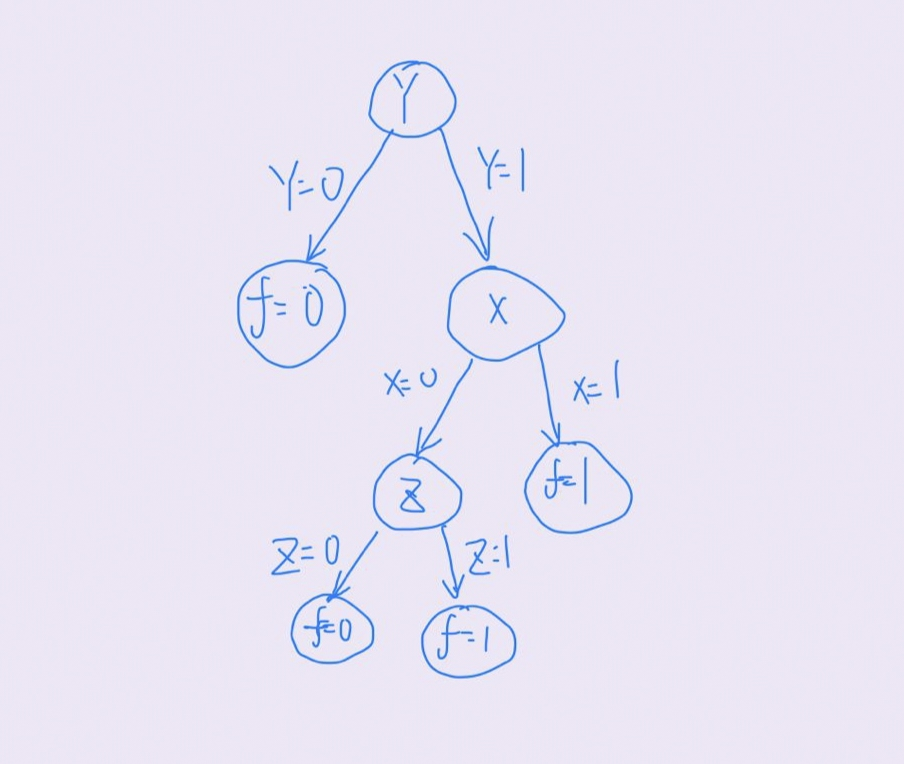
\includegraphics[width=0.8\textwidth,height=0.5\textwidth]{1.jpg}
		\caption{ID3决策树}
	\end{figure} 
	\item[(2)]
	预剪枝: \\
	属性Y划分前精准度为 $\frac{1}{2}$,划分后精准度为 $\frac{2}{3}$,所以应该划分. \\
	属性X划分前精准度为 $\frac{2}{3}$,划分后精准度为 $\frac{2}{3}$,所以不应划分. \\
	\begin{figure}[htbp]
		\centering
		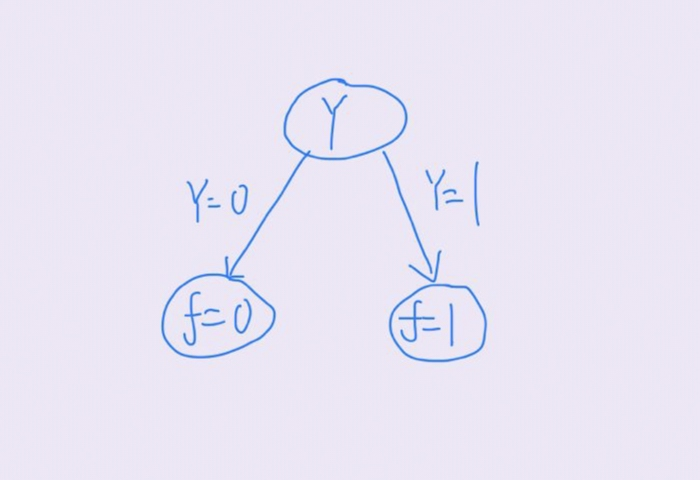
\includegraphics[width=0.8\textwidth,height=0.5\textwidth]{2.jpg}
		\caption{预剪枝决策树}
	\end{figure} 


	后剪枝:\\	
	该决策树在验证集上的精度为 $\frac{5}{6}$. \\
	如果不划分 Z,验证集精度为 $\frac{2}{3}$,所以不进行剪枝.\\
	如果不划分 X,验证集精度为 $\frac{5}{6}$,所以可以不进行剪枝. \\
	如果不划分 Y,验证集精度为 $\frac{1}{2}$,所以不进行剪枝. \\
	\begin{figure}[htbp]
		\centering
		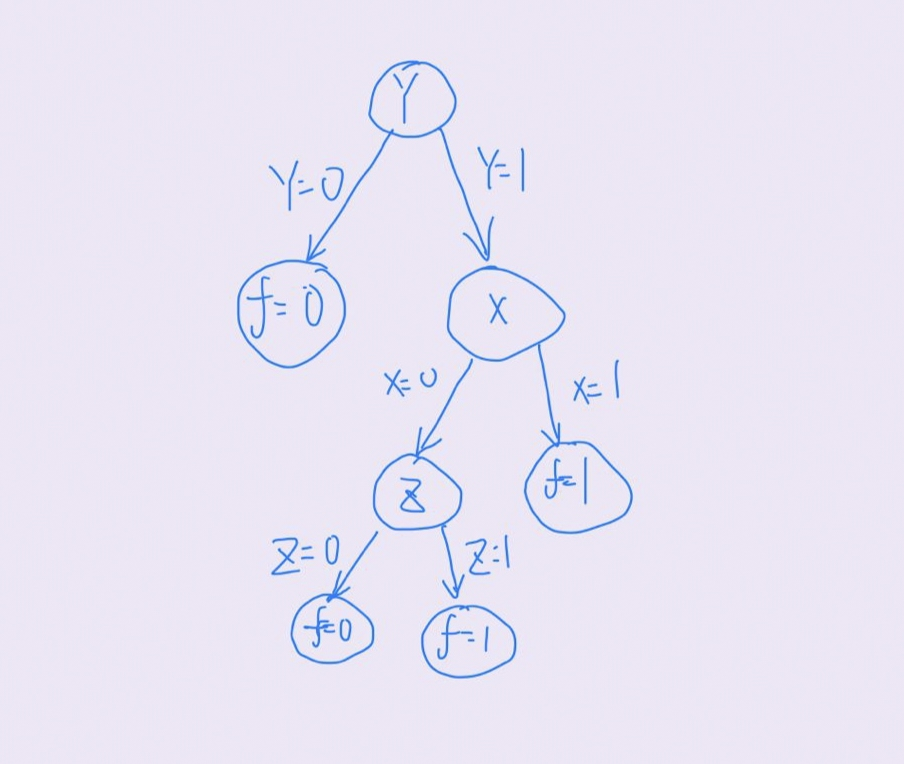
\includegraphics[width=0.8\textwidth,height=0.5\textwidth]{1.jpg}
		\caption{后剪枝决策树}
	\end{figure} 


	\item[(3)]
	预剪枝决策树训练集精度为87.5\%,验证集精度为66\%. \\
	后剪枝决策树训练集精度为100\%,验证集精度为83\%\\
	预剪枝使得决策树的很多分支都没有“展开”,这不仅降低了过拟合的风险,而且减少了决策树的训练时间开销和预测时间开销,但另一方面,
	有些分支的当前划分虽然不能提升泛化性能甚至会降低泛化性能,但是在其基础上进行的后续划分却有可能导致性能显著提高,所以预剪枝有欠拟合的风险。\\
	后剪枝通常比预剪枝保留更多的分支,一般情况下,后剪枝的欠拟合风险很小,泛化性能往往优于预剪枝决策树,但是后剪枝决策树的训练时间开销比预剪枝大得多。
\end{enumerate}
~\\
~\\
~\\
\end{solution}

\newpage

\section{[20pts] Kernel Function}
核函数是 SVM 中常用的工具,其在机器学习中有着广泛的应用与研究. 请自行阅读学习《机器学习》第 6.3 节, 并回答如下问题.
\begin{enumerate}
	\item[(1)] \textbf{[5pts]} 试判断 $\kappa(\x, \z) = \left(\langle\x, \z\rangle - 1\right)^2$ 是否为核函数,并给出证明或反例.
	\item[(2)] \textbf{[5pts]} 试证明:对于半正定矩阵 $\A$,总存在半正定矩阵 $\C$,成立$\A = \C^\top \C$
	\item[(3)] \textbf{[5pts]} 试证明:若 $\kappa_1$ 和 $\kappa_2$ 为核函数, 则两者的直积
	\[
	\kappa_1 \otimes \kappa_2(\x, \z)=\kappa_1(\x, \z) \kappa_2(\x, \z)
	\]
	也是核函数;
	\item[(4)] \textbf{[5pts]} 试证明 $\kappa(\x, \z) = \langle\x, \z\rangle^p$ 对 $\forall p\in\mathbb{Z}_+(p<\infty)$ 均为核函数.

	
\end{enumerate}

\begin{solution}
此处用于写解答(中英文均可)
~\\
~\\
~\\
\begin{enumerate}
	\item[(1)]
	不是核函数. \\
	反例:令数据集$D=\{(1,0), (0,1)\}$ \\
	则$k(x_1, x_1) = 0, k(x_1,x_2) = 1, k(x_2, x_1) = 1, k(x_2, x_2)=0$ \\
	核矩阵:\\
	\begin{equation}
		\left(
		\begin{array}{cc}
			0 & 1 \\
			1 & 0
		\end{array}
		\right)
	\end{equation}
	不是半正定矩阵.
	\item[(2)]
	因为$\A$为半正定矩阵,则其特征值$\lambda_1, \lambda_2,...,\lambda_n$均大于等于0,则存在正交矩阵$\textbf{P}$使得\\
	\begin{equation}
		\begin{aligned} \mathbf{A} & =\mathbf{P} \operatorname{diag}\left\{\lambda_{1}, \lambda_{2}, \ldots, \lambda_{n}\right\} \mathbf{P}^{-1} \\ & =\mathbf{P} \operatorname{diag}\left\{\sqrt{\lambda_{1}}, \sqrt{\lambda_{2}}, \ldots, \sqrt{\lambda}_{n}\right\} \mathbf{P}^{-1} \mathbf{P} \operatorname{diag}\left\{\sqrt{\lambda_{1}}, \sqrt{\lambda_{2}}, \ldots, \sqrt{\lambda}_{n}\right\} \mathbf{P}^{-1} \\ & =\mathbf{P} \operatorname{diag}\left\{\sqrt{\lambda}_{1}, \sqrt{\lambda}_{2}, \ldots, \sqrt{\lambda}_{n}\right\} \mathbf{P}^{-1}\left(\mathbf{P}^{-1}\right) \top \operatorname{diag}\left\{\sqrt{\lambda}_{1}, \sqrt{\lambda}_{2}, \ldots, \sqrt{\lambda}_{n}\right\} \mathbf{P} \\ & =\mathbf{P} \operatorname{diag}\left\{\sqrt{\lambda_{1}}, \sqrt{\lambda}_{2}, \ldots, \sqrt{\lambda}_{n}\right\} \mathbf{P}^{-1}\left(\mathbf{P} \operatorname{diag}\left\{\sqrt{\lambda}_{1}, \sqrt{\lambda}_{2}, \ldots, \sqrt{\lambda}_{n}\right\} \mathbf{P}^{-1}\right) \top\end{aligned}
	\end{equation}
	令 $\mathbf{C}=\mathbf{P}\left\{\sqrt{\lambda}_{1}, \sqrt{\lambda}_{2}, \ldots, \sqrt{\lambda}_{n}\right\} \mathbf{P}^{-1}$, 则$\A=\C^{\top}\C$, $\C$是半正定矩阵。
	\item[(2)]
	$\because A$为半正定矩阵\\
	$\therefore$存在可逆矩阵$D$,使得
	\begin{equation}
		A=D^{T}
		\left(
		\begin{array}{cc}
		E_r & 0  \\
		0 & 0
		\end{array}
		\right)    
		D    
	\end{equation}
	其中$r = rank(A)$\\
	$\therefore $下式成立:\\
	\begin{equation}
		A=D^{T}
		\left(
		\begin{array}{cc}
		E_r & 0  \\
		0 & 0
		\end{array}
		\right)
		\left(
			\begin{array}{cc}
			E_r & 0  \\
			0 & 0
			\end{array}
		\right)    
		D=
		\left(
		\left(
			\begin{array}{cc}
			E_r & 0  \\
			0 & 0
			\end{array}
		\right)
		D
		\right)^{T}
		\left(
		\left(
			\begin{array}{cc}
			E_r & 0  \\
			0 & 0
			\end{array}
		\right)
		D
		\right)
	\end{equation}
	令
	\begin{equation}
		C=
		\left(
			\begin{array}{cc}
			E_r & 0  \\
			0 & 0
			\end{array}
		\right)
		D
	\end{equation}
	则$A=C^{T}C$
	\item[(3)]
	设$K_1,K_2$分别表示$k_1, k_2$的核矩阵\\
	$K=K_1 \otimes K_2$表示$\kappa_1 \otimes \kappa_2(\x, \z)$的核矩阵\\
	\begin{equation}
		\begin{aligned}
			yK^{T}y &= y
			\left(
			\begin{array}{cccc}
				k_1(x_1,z_1)k_2(x_1,z_1) & k_1(x_1,z_2)k_2(x_1,z_2) & ... & k_1(x_1,z_m)k_2(x_1,z_m) \\
				k_1(x_2,z_1)k_2(x_2,z_1) & k_1(x_2,z_2)k_2(x_2,z_2) & ... & k_1(x_1,z_m)k_2(x_1,z_m) \\
				... & ... & ... & ... \\
				k_1(x_m,z_1)k_2(x_m,z_1) & k_1(x_m,z_2)k_2(x_m,z_2) & ... & k_1(x_m,z_m)k_2(x_m,z_m) 
			\end{array}
			\right)
			y^{T} \\
			&= \sum\limits_{i=1}^{m}\sum\limits_{j=1}^{m}k_1(x_i,z_j)k_2(x_i, z_j)y_iy_j \\
			&= tr\left(\left(
				\begin{array}{cccc}
					k_1(x_1,z_1)y_1 & k_1(x_1,z_2)y_1 & ... & k_1(x_1,z_m)y_1 \\
					k_1(x_2,z_1)y_2 & k_1(x_2,z_2)y_2 & ... & k_1(x_1,z_m)y_2 \\
					... & ... & ... & ... \\
					k_1(x_m,z_1)y_m & k_1(x_m,z_2)y_m & ... & k_1(x_m,z_m)y_m 
				\end{array}
			\right)
			\left(
				\begin{array}{cccc}
					k_2(x_1,z_1)y_1 & k_2(x_2,z_1)y_1 & ... & k_2(x_m,z_1)y_1 \\
					k_2(x_1,z_2)y_2 & k_2(x_2,z_2)y_2 & ... & k_2(x_m,z_2)y_2 \\
					... & ... & ... & ... \\
					k_2(x_1,z_m)y_m & k_2(x_2,z_m)y_m & ... & k_2(x_m,z_m)y_m 
				\end{array}
			\right)
			\right) \\
			&= tr\left(
				\left(
					\begin{array}{cccc}
						y_1 &&& \\
						&y_2&& \\
						&&...& \\
						&&&y_m
					\end{array}
				\right)
				K_1
				\left(
					\begin{array}{cccc}
						y_1 &&& \\
						&y_2&& \\
						&&...& \\
						&&&y_m
					\end{array}
				\right)
				K_2^{T}
			\right) \\
		&= tr\left(
			\left(
				\begin{array}{cccc}
					y_1 &&& \\
					&y_2&& \\
					&&...& \\
					&&&y_m
				\end{array}
			\right)
			C^{T}C
			\left(
				\begin{array}{cccc}
					y_1 &&& \\
					&y_2&& \\
					&&...& \\
					&&&y_m
				\end{array}
			\right)
			D^{T}D
		\right)
		\end{aligned}
	\end{equation}
	上式最后一个等式是由于$K_1, K_2$是半正定矩阵,由(2)中结论:\\
	$K_1=C^{T}C, K_2=D^{T}D$ \\
	因为交换矩阵顺序不改变矩阵的迹,所以:\\
	\begin{equation}
		\begin{aligned}
			yK^{T}y &=
			tr\left(
			\left(
				\begin{array}{cccc}
					y_1 &&& \\
					&y_2&& \\
					&&...& \\
					&&&y_m
				\end{array}
			\right)
			C^{T}C
			\left(
				\begin{array}{cccc}
					y_1 &&& \\
					&y_2&& \\
					&&...& \\
					&&&y_m
				\end{array}
			\right)
			D^{T}D
		\right) \\
		&= tr\left(
			\left(
			C
			\left(
				\begin{array}{cccc}
					y_1 &&& \\
					&y_2&& \\
					&&...& \\
					&&&y_m
				\end{array}
			\right)
			D^{T}
			\right)^{T}
			\left(
			C
			\left(
				\begin{array}{cccc}
					y_1 &&& \\
					&y_2&& \\
					&&...& \\
					&&&y_m
				\end{array}
			\right)
			D^{T}
			\right)
		\right) \\
		&= tr(Q^{T}Q)\geq 0
		\end{aligned}
	\end{equation}
	所以$K$半正定,$\kappa_1 \otimes \kappa_2(\x, \z)$是核函数。
	\item[(4)]  
	先证明$p=1$时,$k(x, z) = x^{T}z$是核函数\\
	由核函数的定义,假设输入空间为$\mathcal{X}$\\
	定义映射$\phi: \mathcal{X} \rightarrow \mathcal{H}$ ,
	$\phi (x) = x$ \\
	那么对所有的$x,z\in \mathcal{X}$\\
	$k(x, z) = x^{T}z = \phi (x)\cdot\phi (z)$\\
	所以$k$是核函数\\
	假设当 $p=n-1$的时候,$\kappa(\x,\z) = \langle \x, \z\rangle^p $也是核函数 \\
	由问(3)得到的结论
	当 $p=n$的时候,$\kappa(\x,\z) = \kappa_{n-1} \bigotimes \kappa_1 (\x,\z) = \langle \x, \z\rangle^{n-1} \cdot \langle \x, \z\rangle $,所以 $p=n$时也是核函数. \\
	数学归纳法成立,$\kappa(\x, \z) = \langle\x, \z\rangle^p$ 对 $\forall p\in\mathbb{Z}_+(p<\infty)$ 均为核函数.
\end{enumerate}
\end{solution}



\end{document}